%%%%%%%%%%%%%%%%%%%%%%%%%
%% Template for small reports
%%%%%%%%%%%%%%%%%%%%%%%%%

\documentclass[letterpaper,notitlepage,11pt]{article}

%Additional packages
\usepackage{fullpage} %For using small margins 
\usepackage{latexsym}
\usepackage{amssymb}
\usepackage{amsmath}
\usepackage[english]{babel}
\usepackage[pdftex]{color,graphicx} %Images for pdfs
\usepackage[pdftex,colorlinks]{hyperref} %Hyperlinked pdfs
\usepackage{listings} %For adding code

%If you need to add math
\newenvironment{proof}{\begin{trivlist} \item[] {\em Proof:}}{\hfill $\Box$ \end{trivlist}}
\newtheorem{theorem}     {Theorem}
\newtheorem{lemma}       {Lema}
\newtheorem{observation} {Observation}
\newtheorem{proposition} {Proposition}
\newtheorem{conjecture}  {Conjecture}
\newtheorem{corollary}   {Corolari}
\newtheorem{property}    {Property}
\newtheorem{definition}  {Definition}

%Title box
\newcommand{\titlebox}[6]
{\noindent\fbox{\parbox{\textwidth}{#1 \hfill\textbf{#2}\begin{center} 
\LARGE #3 \end{center}#4 $<$\href{mailto:#5}{#5}$>$ \hfill #6}}\bigskip\\}

%If you want to include code
%standard configuration of the listings package
%\lstset{language=matlab, basicstyle=\footnotesize, numbers=left, frame=lines, frameround=tfft,breaklines=true}
%how to include a file "\lstinputlisting{../../Courses/16720-CV/hw2/matlab/blockify.m}"


%%%%%%%%%%%%%%%%%%%%%%
%% Here begins the document
%%%%%%%%%%%%%%%%%%%%%%
\begin{document}
\titlebox
{CMU  - Robotics Institute}                           % Institution (ex: CMU - Robotics Institute)
{Manipulation Lab - Simple Hands Project}    % Center (ex: Manipulation Lab)
{Hand node - ROS - Introduction}               % Title
{}                                                                   % Author
{manipulationLab@gmail.edu}                       % e-mail
{\today}                                                         % Date (format yyyy/mm/dd)


\section{Hand}
Hand\_node is a ROS interface to control the gripper in the Simple
Hands project implemented in C++. It provides abstraction to command
the motor controller of the hand and read the finger encoders through
an Arduino microcontroller.

\begin{figure}[h]
  \centering 
  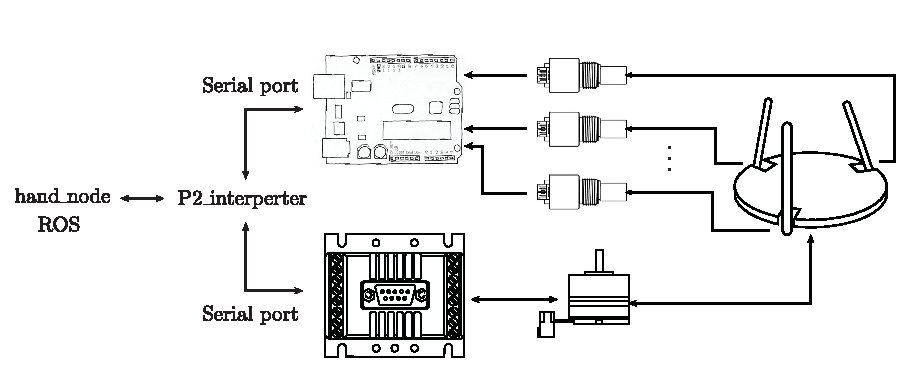
\includegraphics{figures/schematic}
  \caption{Schematic of the control of the hand.}
  \label{fig:handControlSchematic}
\end{figure}

It is composed of two ROS packages: hand\_node, a standalone typical
ROS package that provides topics and services, and hand\_comm,
including the message definitions and a C++ client class to simplify
the invocation and communication with hand\_node.

\subsection{hand\_node}
\noindent (Located at \url{svnroot/code/nodes/hand/ROS/hand_node})
\\

\textbf{\underline{Services:}}

\begin{itemize}
\item \textbf{hand\_Calibrate}: Blocking service to calibrate the motor
  encoder. The hand opens until reaching a hard stop and homes the
  motor at that position (motor encoder set to 0). This service needs
  to be called every time that the hand is switched on, since the
  motor encoder is not absolute and loses the encoder count when
  disconnected.

\begin{verbatim}
---
int64 encMotor   # Motor encoder
int64[] enc      # List of finger encoders
int64 ret        # Set to 1 (success) or 0 (error)
string msg       # Error description
\end{verbatim}

\item \textbf{hand\_SetForce}: Service to set the max force that the
  hand should be using when opening or closing. Internally, this
  service limits the max current that the motor should use. The input
  parameter force should be a real value between 0 and 1. That value
  will be mapped to a current value between system parameters
  minIntensity and maxIntensity.

\begin{verbatim}
float64 force # value from 0 to 1
---
int64 ret     # Set to 1 (success) or 0 (error)
string msg    # Error description
\end{verbatim}

\item \textbf{hand\_SetSpeed}: Service to set the speed of the
  hand. Internally, this service sets the speed of the hand motor. the
  input parameter speed should be a real value between 0 and 1.  That
  value is mapped to a speed value between system parameters minSpeed
  and maxSpeed.

\begin{verbatim}
float64 speed    # Value between 0 and 1
---
int64 ret        # Set to 1 (success) or 0 (error)
string msg       # Error description
\end{verbatim}

\item \textbf{hand\_GetEncoders}: Service to get the value of the
  motor and finger encoders.

\begin{verbatim}
---
int64 encMotor      # Motor encoder
int64[] encFinger   # finger encoders
int64 ret           # Set to 1 (success) or 0 (error)
string msg          # Error description
\end{verbatim}

\item \textbf{hand\_GetAngles}: If the hand is calibrated, this
  service returns the value of the angles of the motor and fingers.

\begin{verbatim}
---
float64 angleMotor   # Motor angle
float64[] angle      # Finger angles
int64 ret            # Set to 1 (success) or 0 (error)
string msg           # Error description
\end{verbatim}

\item \textbf{hand\_SetEncoder}: Non-blocking service to set the command the
  position of the motor encoder.

\begin{verbatim}
int64 enc      # Position of the motor encoder
---
int64 ret      # Set to 1 (success) or 0 (error)
string msg     # Error description
\end{verbatim}

\item \textbf{hand\_SetAngle}: Non-blocking service to set the command the
  position of the motor angle, if the hand is calibrated.

\begin{verbatim}
float64 angle   # Nominal position of the motor.
                # 0.0 sets the fingers perpendicular to the palm.
---
int64 ret       # Set to 1 (success) or 0 (error)
string msg      # Error description
\end{verbatim}

\item \textbf{hand\_Ping}: Service to ping the hand and check if motor
  and encoders are available.

\begin{verbatim}
---
int64 ret      # Set to 1 (success) or 0 (error)
string msg     # Error description
\end{verbatim}

\item \textbf{hand\_SetRest}: Service to stop the hand motor. Even if
  the hand is not moving, the motor controller is actively controlling
  the motor positions to recover form any external deviations. It is
  good practice to set the motor to rest when we no longer care, in
  order to avoid overheating of the motor.

\begin{verbatim}
---
int64 ret     # Set to 1 (success) or 0 (error)
string msg    # Error description
\end{verbatim}

\item \textbf{hand\_WaitRest}: Blocking service to wait until the hand
  stops. The hand stops when it gets to the commanded motor position,
  or when it gets stuck before getting there for more than half a
  second. Delay is an input parameter that specifies how long the
  service should wait until checking for the hand to be stopped. This
  is useful, for example when we issue a hand\_WaitRest right after a
  hand\_SetEncoder, since it takes a while for the hand to start
  moving.

\begin{verbatim}
float64 delay    # Seconds to wait before begin to check for rest
---
int64 ret        # Set to 1 (success) or 0 (error)
string msg       # Error description
\end{verbatim}

\item \textbf{hand\_IsMoving}: Service to check whether the hand is
  moving or not.

\begin{verbatim}
---
int64 moving     # 1 (moving) 0 (not)
int64 ret        # Set to 1 (success) or 0 (error)
string msg       # Error description
\end{verbatim}
\end{itemize}


\textbf{\underline{Topics:}}

\begin{itemize}
\item \textbf{hand\_EncodersLog}: Topic broadcasted at 40Hz with the
  motor and finger encoder values.

\begin{verbatim}
float64 timeStamp    # ROS time-stamp
int64 encMotor       # Motor encoder
int64[] encFinger    # Finger encoders
\end{verbatim}

\item \textbf{hand\_AnglesLog}: Topic broadcasted at 40Hz with the
  motor and finger angles. Only published when the hand is calibrated.

\begin{verbatim}
float64 timeStamp      # ROS time-stamp
float64 angleMotor     # Motor angle
float64[] angle        # Finger angles
\end{verbatim}
\end{itemize}

\subsection{hand\_comm}
\noindent (Located at \url{svnroot/code/nodes/hand/ROS/hand_comm})

\noindent Hand\_comm is a ROS wrapped C++ class meant to simplify the
communication with hand\_node. It contains:

\begin{enumerate}
\item Message and Service definitions. When creating a ROS application
  that uses hand\_node, the application only needs to be dependent
  on hand\_comm. As a consequence, the application does not need to
  link to all the drivers and libraries needed to control the hand. 
\item C++ class HandComm that handles all configuration and
  initialization required to use hand\_node. As an example, if we want
  to call the service hand\_Ping, we only need instantiate a HandComm
  object and call to the member routine handPing. Otherwise
  we would have to include all required header files, subscribe to the
  hand\_Ping service and format the required message to be sent to the
  service.
\end{enumerate}

\textbf{\underline{Usage example:}}

\begin{verbatim}
  ...
  ros::NodeHandle node;
 
  HandComm hand;           //Create HandComm client
  hand.subscribe(&node);   //Subscribe to all services of hand_node
  while(!hand.Ping());     //Wait until hand is ready to move
  hand.Calibrate();        //Calibrate the hand.

  ...
\end{verbatim}


\textbf{\underline{Member routines}}:

\begin{verbatim}

class HandComm
{
  public:

    HandComm();
    HandComm(ros::NodeHandle* np);
    ~HandComm();

    // Subscribe Function
    void subscribe(ros::NodeHandle* np);

    // Subscribe to Topics
    void subscribeAngles(ros::NodeHandle* np, int q_len, 
        void (*funcPtr)(const hand_comm::hand_AnglesLogConstPtr&));
    void subscribeEncoders(ros::NodeHandle* np, int q_len, 
        void (*funcPtr)(const hand_comm::hand_EncodersLogConstPtr&));

    // Shutdown service clients
    void shutdown();

    bool Ping();
    bool Calibrate();
    bool GetAngles(double &mot_ang, double ang[NUM_FINGERS]);
    bool GetAngles(double &mot_ang, Vec &ang);
    bool IsMoving(bool &moving);
    bool SetEncoder(int enc);
    bool SetRest();
    bool WaitRest(int delay);
    bool GetEncoders(int &mot_enc, int enc[NUM_FINGERS]);
    bool GetEncoders(int &mot_enc, Vec &enc);
    bool SetAngle(double angle);
    bool SetForce(double force);
    bool SetSpeed(double speed);

  private:
...
};

\end{verbatim}


%%%%%%%%%%%%%%%%%%%%
%% If you want bibliography
%%%%%%%%%%%%%%%%%%%%
%\bibliographystyle{unsrt}
%\bibliography{} %Name and location of the bibfile

%To cite a reference -> \cite{cite_name}
%To make a reference appear in the bibliography without a citation in the text -> \nocite{cite_name}

\end{document}
